\documentclass[answers,addpoints,11pt]{exam}
\usepackage[utf8]{inputenc}
\usepackage[english]{babel}
\usepackage{listings}
\usepackage{amsmath}
\usepackage{algpseudocode}
\usepackage{graphicx}
\usepackage{amssymb}
\usepackage{amsthm}
\usepackage{hyperref}
\usepackage{logicproof}
\usepackage{multicol}
\usepackage{environ}
\usepackage{xcolor}
\usepackage{qtree}

\newcommand{\limit}[1]{ \lim_{n \rightarrow \infty} \left( #1 \right) }
\bracketedpoints
\qformat{Question \thequestion{} : \totalpoints{} \points \hfill}

%These setting will make the code areas look Pretty
\lstset{
	escapechar=~,
	numbers=left, 
	%numberstyle=\tiny, 
	stepnumber=1, 
	firstnumber=1,
	%numbersep=5pt,
	language=C,
	stringstyle=\ttfamily,
	%basicstyle=\footnotesize, 
	showstringspaces=false,
	frame=single
}

\title{CS260 - Data Structures - Written Assignment 1}
\author{Fitsum Alebachew} 
\date{}

\begin{document}
\maketitle

\vspace{-0.5in}
\begin{questions}
%%%%%%%%%%%%%%%%%%%%%%%%%%
%%%% Question 1 %%%%%%%%%%
%%%%%%%%%%%%%%%%%%%%%%%%%%
\question

Determine the most accurate $\Theta(\cdots)$ for each function and explain how you calculated the tight bound. Assume that the functions take an input array of size $n$. 

\vspace{0.25in}


\begin{parts}

\part[3] The {\tt max} method is $\Theta(\hspace{1 pc})$.

\begin{lstlisting}
int max(int* a, int size)
{
    if(size < 2)
    	return -1;
    if(a[0] > a[1])
        return a[0];
    else
        return a[1];
}
\end{lstlisting}

\begin{solution}
This will do a maximum of 2 comparisons. It is $\Theta(1)$.
\end{solution}

\part[3] The {\tt maxElement} method is $\Theta(\hspace{1 pc})$.

\begin{lstlisting}
int maxElement(int* a, int size)
{
    int max = a[0];
    for(int i=1; i<size; i++)
        if(a[i] > max)
            max = a[i];
    return max;
}
\end{lstlisting}

\begin{solution}
This will iterate through the list once. It is $\Theta(n)$.
\end{solution}

\part[4] The {\tt maxSubseqSum} method is $\Theta(\hspace{1 pc})$.

\begin{lstlisting}
int maxSubseqSum(int* a, int size)
{
    max=a[0];
    for(int i=1; i<size; i++)
    {
        sum = 0
        for(int j=i; j<size; j++)
        {
            sum+=a[j];
            if(sum > max)
                max=sum;
        }
    }
    return max;
}
\end{lstlisting}

\begin{solution}
In the nested for loop, for each initial iteration in the list, it iterates through the whole list again. That makes it $\Theta(n^2)$.
\end{solution}

\end{parts}

%%You can use \newpage to start a new page
\newpage
%%%%%%%%%%%%%%%%%%%%%%%%%%
%%%% Question 2 %%%%%%%%%%
%%%%%%%%%%%%%%%%%%%%%%%%%%
\question[10]
    Consider the following functions: 
    \begin{itemize}
        \item $\log_2x$
        \item $x\cdot \log_2x$
        \item $(3/2)^x$
        \item $x/\log_2x$
        \item $2^x$
        \item $\sqrt{x}$
        \item $x^2$
        \item $(\log_2x)^2$
        \item $(1/3)^x$
    \end{itemize}
    
    You are told that, functions above represent the number of operations carried out by a set of algorithms that do the same job, albeit in different ways. Order the functions from slowest growth rate to the fastest growth rate (i.e., sort the algorithms from fastest to slowest). Explain your reasoning for consecutively ordered functions, possibly by using the limit method, to get credit.

\begin{solution}
$(1/3)^x < \log_2(x) < (\log_2(x))^2 < \sqrt x < x/\log_2x < x < x \cdot \log_2(x) < x^2 < 2^x$.\\\\
$(1/3)^x$ is a decreasing function, so it will have a negative growth rate. The second growing functions are the log functions(ordered by degree). Even powered to any number, they grow slower than squareroot functions of any degree. Then the polynomials ordered to their degree or the lesser growing functions they're being multiplied/divided by if they have the same degrees. Then exponentials, which grow faster than polynomials.

\end{solution}

%%%%%%%%%%%%%%%%%%%%%%%%%%
%%%% Question 3 %%%%%%%%%%
%%%%%%%%%%%%%%%%%%%%%%%%%%
\question
Professor Bond has developed the following algorithm that he claims is going to be a break through in computer science. 

Assuming array is zero indexed, A[0] is the first and A[n-1] is the last element, the algorithm is as follows:
 \begin{lstlisting}
mysteryFunction(A, n)
{
   int lastPos=n-1;
   while(lastPos > 0)
   {
      int maxPos=0;
      for(int i=0; i <= lastPos; i++)
         if(A[i] > A[maxPos])
            maxPos = i;
      swap(A, maxPos, lastPos);
      lastPos = lastPos - 1;
   }
}
 \end{lstlisting}
 
\begin{parts}
 \part[2] Explain what the algorithm does in plain English.
\begin{solution}
It finds the maximum element, swaps it to the end of the array, then does the same for the remainder of the list until the whole list is sorted.
\end{solution}

 \part[2] Why does the algorithm run for all elements but the last, rather than for all elements?
 \begin{solution}
After the first run, the last element is sorted and also the largest in the array, so for the algorithm to work, it needs to exclude it from the comparing process.
\end{solution}

 \part[3] What is the best case of this algorithm and what is its best case running time in $\Theta$ notation?
 \begin{solution}
The algorithm must run through each element going down by one for each iteration $(1 + 2 + 3 + ... + n) = n(n+1)/2$. This is $\Theta(n^2)$.
\end{solution}

 \part[3] What is the worst case of this algorithm and what is its worst case running time in $\Theta$ notation?
 \begin{solution}
The algorithm will run through each element going down by one for each iteration $(1 + 2 + 3 + ... + n) = n(n+1)/2$. This is $\Theta(n^2)$. The same! The kind of input, like presorting does not change the run time, only the size of input matters.
\end{solution}

\end{parts}

%%%%%%%%%%%%%%%%%%%%%%%%%%
%%%% Question 4 %%%%%%%%%%
%%%%%%%%%%%%%%%%%%%%%%%%%%
\question

Professor Holmes came up with the idea of a sorting algorithm that he calls {\it Trinary Sort} which he claims is asymptotically faster than merge sort, despite being similar in logic. Unlike merge sort, trinary sort splits the input list into three roughly equal parts at each step of the recursion as long as the list is splittable (i.e., has at least 3 elements in this case). The merge operation, similar to what it does in mergeSort, takes three already sorted subarrays, and merges them.

\begin{parts}
 \part[4] In merge sort, merge operation takes make $n-1$ comparisons in total to merge two lists of size $n/2$, which takes $O(n)$ time. How many comparisons will the merge operation of Trinary sort make to merge three sublists of size $(n/3)$? What would be the asymptotic bound?
 
 \begin{solution}
When merging 3 sublists into one, two comparisons will have to be made to find the largest out of three values. The total number of comparisons will be $2n - 3$ since the last two elements will need 1 or no comparisons needed. This is also $\Theta(n)$.
\end{solution}

 \part[5] What is the total running time of the Trinary Search algorithm? Show it using the {\bf tree expansion method} as we have done in the class.\\
 \begin{solution}

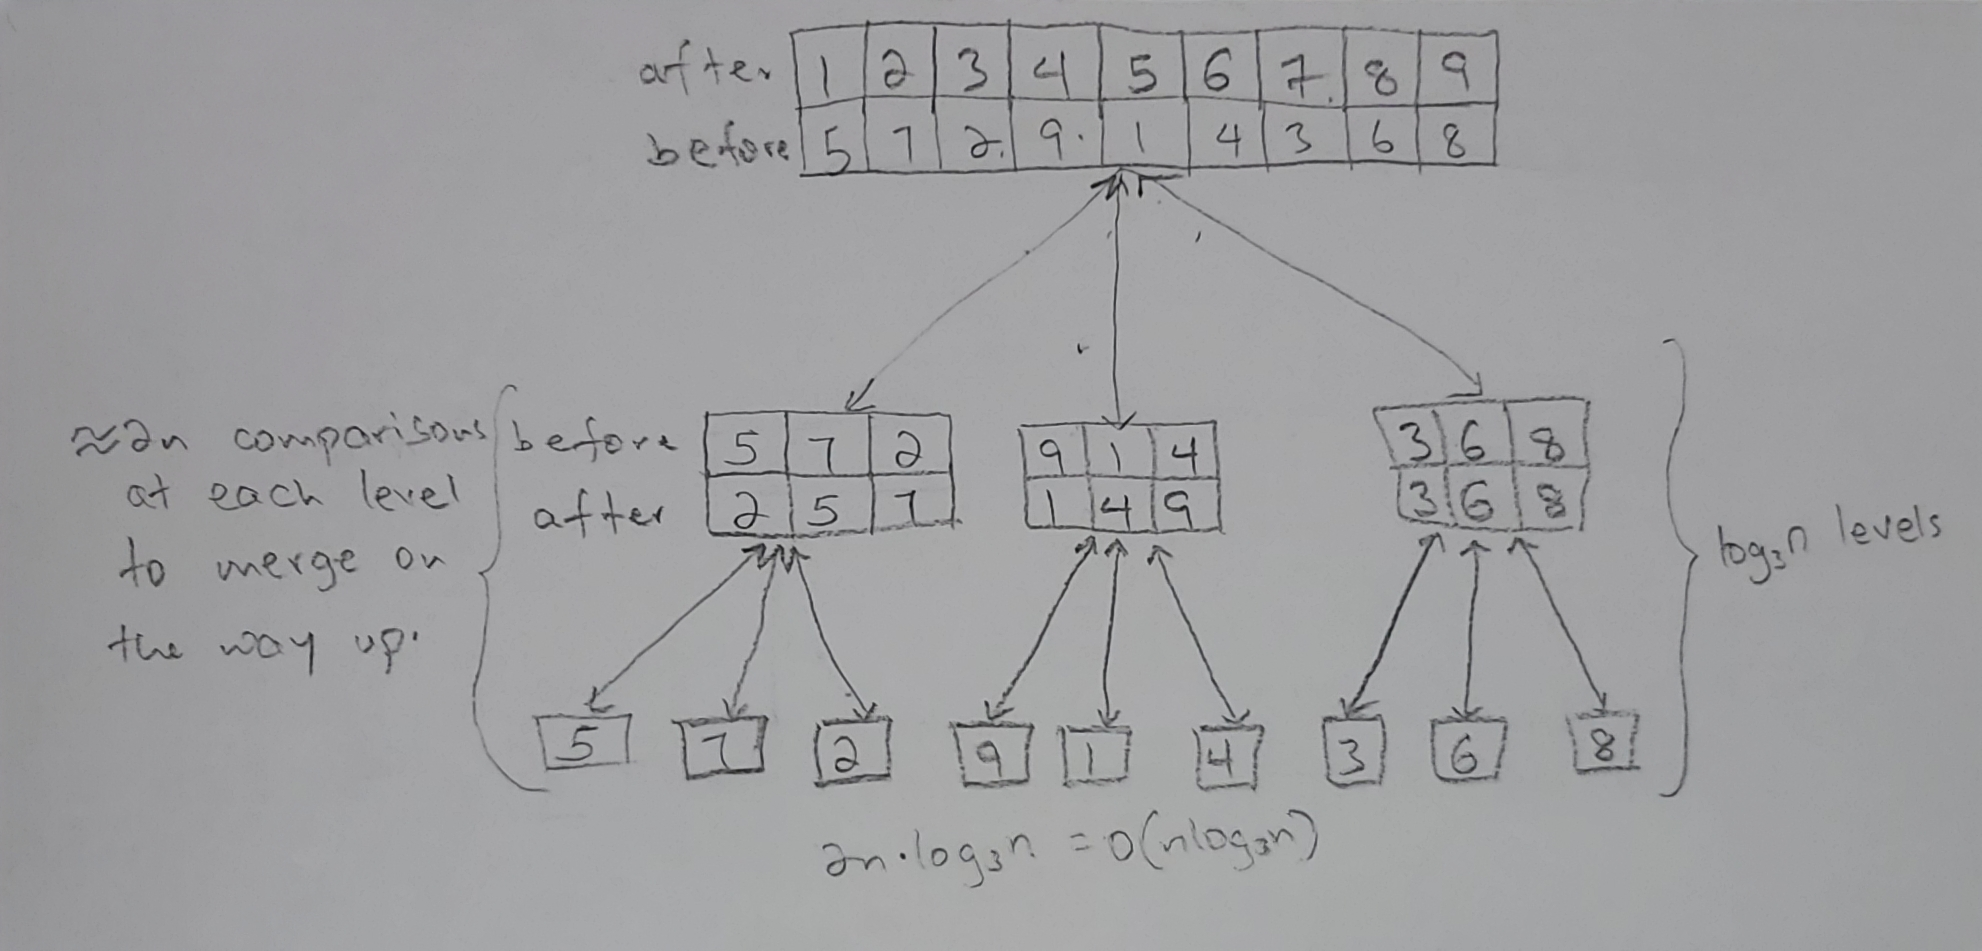
\includegraphics[scale=0.2]{tree.jpg}
\end{solution}
 
 \part[2] What is the recurrence relation for the Trinary Search algorithm? 
 \begin{solution}
$T(n) = 3T(n/3) + 2n$
\end{solution}

 \part[4] Calculate the total running time of Trinary search, this time by {\bf expanding the recurrence relation} you suggested above.
 \begin{solution}
$T(n) = O(n\log_3n)$.
\end{solution}
 
 \part[5] Is Professor Holmes right in his claim that Trinary search is asymptotically faster than Merge Sort? Why/why not? Prove your point. (Hint: Use limit method that was suggested in class and exemplified in the exercise posted, to compare upper/lower bounds for algorithms)
 \begin{solution}
No. Both of their runtimes are asymptotically equivalent, because $\log_3n$ and $\log_2n$ are only different by a constant multiple ($\log_3n/\log_2n = \log2/\log3$).
\end{solution}
 
\end{parts}


%%%%%%%%%%%%%%%%%%%%%%%%%%
%%%% Question 5 %%%%%%%%%%
%%%%%%%%%%%%%%%%%%%%%%%%%%
\question
Calculate an upper bound (tight bound, if possible) for each of the following recurrence relations. Show your work by expanding the relation as was done in class.

\begin{parts}
\part[5] $T(n) = T(n-1) + n$
\begin{solution}
$T(n) = T(n-2) + 2n = T(n-3)+3n = T(n-k)+kn$\\
Stopping condition: $k=n-1$\\
$T(n)=T(1)+n(n-1) = n^2 -n + 1 = \Theta(n^2)$
\end{solution}


\part[5] $T(n) = T(n/2) + 1$
\begin{solution}
$T(n) = T(n/4)+2 = T(n/8)+3 = T(n/2^k)+k$\\
Stopping condition: $2^k = n, k = \log_2n$\\
$T(n) = T(1) + log_2n = 1 + log_2n = \Theta(log_2n)$

\end{solution}

\part[5] $T(n) = 4T(n/3) + n$
\begin{solution}
$T(n)=4(4T(n/9) + n/3) + n = 16T(n/9) + 7n/3\\
= 4(4(4T(n/27)+n/9)+n/3)+n = 64T(n/27) + 37n/9\\
=4^kT(n/3^k)+n((4/3)^{k-1}+(4/3)^{k-2}+...+1)$\\
Stopping condition: $n = 3^k, k = \log_3n$\\
$T(n)=c_1n+c_2n\log_3n$ where c's are constants independent of n $=\Theta(n\log_3n)$
\end{solution}
\end{parts}
%%%%%%%%%%%%%%%%%%%%%%%%%%
%%%% Question 6 %%%%%%%%%%
%%%%%%%%%%%%%%%%%%%%%%%%%%
\question
You applied to Google for an internship and they wanted to test your abilities to come up with novel data structures. The company is currently developing tiny robots that has very limited memory and computational resources. They are in need of data structures to be used in embedded system implementation of the robot. Since it is easier to handle and process arrays than linked lists, the company want {\bf the data structures to be array based}, which will be desirable for a limited system. Answer the questions below accordingly.

\begin{parts}
\part[5] You are being asked to design a new stack that Google wants to name as {\it Amphisbaena} (why on earth would they want to call it such a weird name!!). Amphisbaena will actually be two stacks on a single array of size $n$, without the two overflowing each other unless there are $n$ elements in total among both stacks. In plain English, explain a data structure that will dynamically and efficiently hold two stacks together in a single structure.
\begin{solution}
Two stacks can be implemented on a single array if one begins from the start of the array and one from the end. Elements pushed and popped are done so accordingly using two stack pointers pointing to the top of each stack. When the pointers point to adjacent locations, the array will have a combined n elements and is full.
\end{solution}

\part[5] You need to design a queue, weirdly enough named as {\it Ourobors}, to be used in the robot's operating system. Since, the runtime of dequeue operation of a standard queue would be inefficient for the robot, Ouroboros should support a constant time dequeue operation. In plain English, suggest and explain such a queue structure.\\

\begin{solution}
We can implement a circular array where added elements don't need to be shifted, but the front and rear pointers are shifted to the necessary locations when an item is added or removed. With this implementation, the dequeue operation will have a runtime of $O(1)$.
\end{solution}

\end{parts}

%%%%%%%%%%%%%%%%%%%%%%%%%%
%%%% Question 7 %%%%%%%%%%
%%%%%%%%%%%%%%%%%%%%%%%%%%
\question
Your interview at Google was not too bad, and you are expecting to hear from them for a second interview. While waiting for it, thinking that it will not hurt to have alternatives at hand, you applied for an internship at Microsoft. They gave you a singly linked list where there is a pointer that points to the head of the list, and each element of the list points to the next element (as is the case in singly linked lists), with the exception of last element pointing to NIL. They are asking you to develop a function called {\it reverse} that takes the list as input and reverses the order of objects in $O(n)$ time while using $O(1)$ amount of extra memory.

\begin{parts}
\part[5] Write the pseudocode of your {\it reverse} function.
\begin{solution}
\begin{lstlisting}
reverse(node **head){
    node *next, *prev = NULL;
    for (node *cur = *head; cur != NULL;cur = next){
        next=cur->next;
        cur->next = prev;
        prev = cur;
    }
    *head = prev;
} 
\end{lstlisting}
\end{solution}

\part[5] Explain the running time of your algorithm.
\begin{solution}
The algorithm runs through the linked list once and uses two additional variables to keep track of next and previous nodes since we are changing the next values in the iterations. This gives it the required $O(n)$ running time and $O(1)$ extra memory usage.
\end{solution}

\end{parts}
%%%%%%%%%%%%%%%%%%%%%%%%%%
%%%% Question 8 %%%%%%%%%%
%%%%%%%%%%%%%%%%%%%%%%%%%%
\question[5]
Dictionaries are data structures specialized in storing, finding, and removing records from the collection, that keeps record of {\bf unique} elements. You are being asked to design a a dictionary data structure for a specific input set, where you are guaranteed that the input set is going to be integers drawn from the range [1,k] for some some finite integer n. Design a data structure where search, insertion, and deletion operations are done in O(1) time in the worst case.  (Note: initialization can take O(n) time)

\begin{solution}
We can use a hash table where each value has a key determined by a hash function. Inserting, searching and deleting will take $O(1)$ time since the hashing function will give us the address of the element in focus. When there are collisions, the dictionary can be rehashed (initialized again) to a bigger size until there are no collisions.
\end{solution}

%%%%%%%%%%%%%%%%%%%%%%%%%%
%%%% Question 9 %%%%%%%%%%
%%%%%%%%%%%%%%%%%%%%%%%%%%
\question
You got an offer letter from Google for your internship and accepted it without thinking too much... very soon to realize that this was the beginning of a nightmare (as they will keep asking you challenging algorithms questions throughout your internship)!! Your group leader wants to test your knowledge on hash tables as well as your algorithm design skills with the following question: We have a list of unique integers. We would like to find whether there exist two pairs of integers, such that their summations are equal, To be more precise, determine whether there exists pairs (p, q) and (r, t) in the list which satisfies p+q = r+t. You can print any such pairs if there exists more than one correct answer.  
\begin{parts}
 \part[5] A naive algorithm to solve this problem can achieve $O(n^4)$ run time. In your own words, explain such a naive approach that will do the job.
 \begin{solution}
We can write a quadruple nested for loop to check the combination of every two pairs of numbers against eachother. The first two loops would loop through p and q values, and the other two will loop through r and t values.
\end{solution}

 \part[5] Using ha data structure that would allow a better performance, suggest a $O(n^2)$ run time algorithm that tackles the problem.
 \begin{solution}
A run through the list can be done to find every sum value of possible two number pairs and store that in a dictionary data structure, this takes $O(n^2)$ time. While storing the values, we can check if the sum is a member of the dictionary(which is done either way). If matches are found, they can be stored in a list holding the matches and returned to the user.
\end{solution}

\end{parts}

\end{questions}
\end{document}
